\documentclass[10pt,twoside,slovak,a4paper]{article}

\usepackage[slovak]{babel}
\usepackage[IL2]{fontenc}
\usepackage[utf8]{inputenc}
\usepackage{graphicx}
\usepackage{url}
\usepackage{hyperref}
\usepackage[final]{pdfpages}

\usepackage{cite}

\pagestyle{headings}

\title{Životný cyklus softvérového testovania – jeho fázy, ciele a priority
\thanks{: Ing. Ján Lúčanský}} % meno a priezvisko vyučujúceho na cvičeniach

\author{Stanislav Krištof\\[2pt]
	{\small Slovenská technická univerzita v Bratislave}\\
	{\small Fakulta informatiky a informačných technológií}\\
	{\small \texttt{xkristof@stuba.sk}}
	}

\date{\small 14. október 2021} % upravte



\begin{document}

\maketitle
%\makethanks
\begin{abstract}
\ldots
\end{abstract}



\section{Úvod}
Tento článok sa bude zaoberať modelom, ktorého existencia je kľúčová pre vývoj softvéru a 
softvérové inžinierstvo všeobecne – životným cyklom softvérového testovania. Aj napriek tomu, že 
v rôznych spoločnostiach má tento model rôznu podobu, základná štruktúra zostáva viacmenej 
rovnaká. V článku si vysvetlíme, z ktorých jednotlivých fáz sa životný cyklus softvérového 
testovania skladá. Dozvieme sa, aké sú aktivity spojené s jednotlivými fázami cyklu. Článok sa 
taktiež bude zameriavať na rôzne druhy testovania (white box testing, black box testing, static 
testing...) a ich využitie v jednotlivých fázach vývoja softvéru a na cieľ a priority softvérového 
testovania.

Čo znamená slovo testovanie, jeho ciele a priority si vysvetlíme v časti ~\ref{testovanie}.
Definíciu životného cyklu softvérového testovania a ako vyzerá si vystvetlíme v časti ~\ref{diagram}.
O jednotlivých druhoch softvérového testovania sa porozprávame v ~\ref{dolezita} a~\ref{dolezitejsia}.
Záverečné poznámky prináša časť~\ref{zaver}.



\section{Testovanie} \label{testovanie}

\begin{figure*}[tbh]
\centering
Testovanie softvéru je dôležitou a neoddeliteľnou časťou
\end{figure*}


\section{Životný cyklus softvérového testovania} \label{diagram}

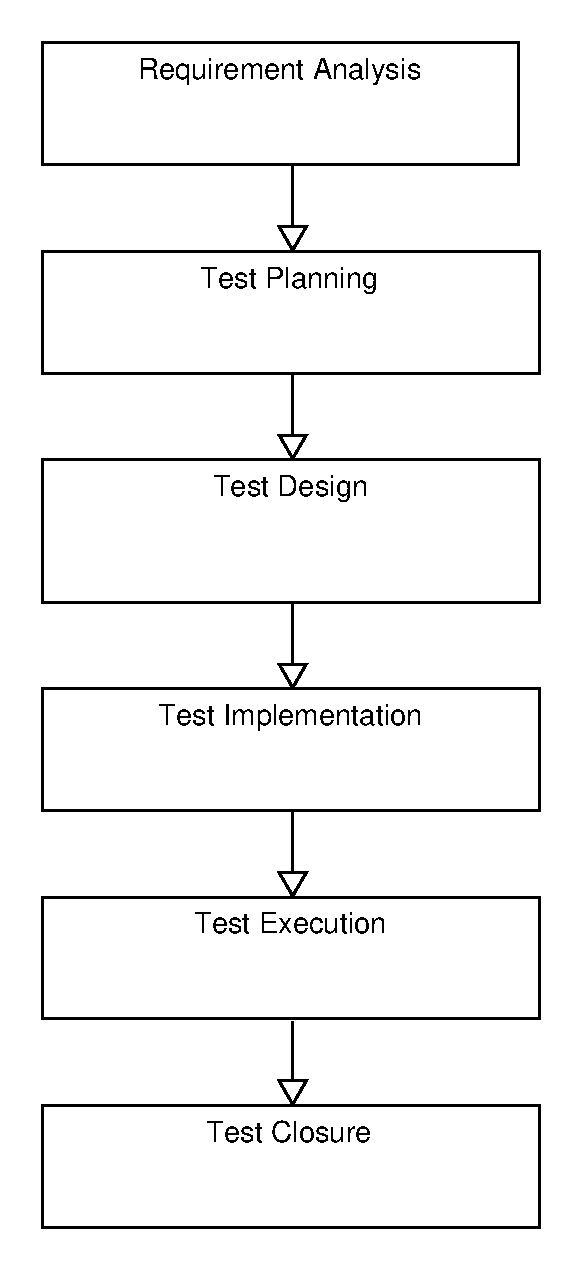
\includepdf[pages=-,pagecommand={},width=\textwidth, height=500pt]{STLC-diagram.pdf}


Z obr.~\ref{f:rozhod} je všetko jasné. 

\begin{figure*}[tbh]
\centering
%\includegraphics[scale=1.0]{diagram.pdf}
Aj text môže byť prezentovaný ako obrázok. Stane sa z neho označný plávajúci objekt. Po vytvorení diagramu zrušte znak \texttt{\%} pred príkazom \verb|\includegraphics| označte tento riadok ako komentár (tiež pomocou znaku \texttt{\%}).
\caption{Rozhodujúci argument.}
\label{f:rozhod}
\end{figure*}



\section{Iná časť} \label{ina}

Základným problémom je teda\ldots{} Najprv sa pozrieme na nejaké vysvetlenie (časť~\ref{ina:nejake}), a potom na ešte nejaké (časť~\ref{ina:nejake}).\footnote{Niekedy môžete potrebovať aj poznámku pod čiarou.}

Môže sa zdať, že problém vlastne nejestvuje\cite{Coplien:MPD}, ale bolo dokázané, že to tak nie je~\cite{Czarnecki:Staged, Czarnecki:Progress}. Napriek tomu, aj dnes na webe narazíme na všelijaké pochybné názory\cite{PLP-Framework}. Dôležité veci možno \emph{zdôrazniť kurzívou}.


\subsection{Nejaké vysvetlenie} \label{ina:nejake}

Niekedy treba uviesť zoznam:

\begin{itemize}
\item jedna vec
\item druhá vec
	\begin{itemize}
	\item x
	\item y
	\end{itemize}
\end{itemize}

Ten istý zoznam, len číslovaný:

\begin{enumerate}
\item jedna vec
\item druhá vec
	\begin{enumerate}
	\item x
	\item y
	\end{enumerate}
\end{enumerate}


\subsection{Ešte nejaké vysvetlenie} \label{ina:este}

\paragraph{Veľmi dôležitá poznámka.}
Niekedy je potrebné nadpisom označiť odsek. Text pokračuje hneď za nadpisom.



\section{Dôležitá časť} \label{dolezita}




\section{Ešte dôležitejšia časť} \label{dolezitejsia}




\section{Záver} \label{zaver} % prípadne iný variant názvu



%\acknowledgement{Ak niekomu chcete poďakovať\ldots}


% týmto sa generuje zoznam literatúry z obsahu súboru literatura.bib podľa toho, na čo sa v článku odkazujete
%\bibliography{literatura}
%\bibliographystyle{plain} % prípadne alpha, abbrv alebo hociktorý iný
\end{document}
